\documentclass[a4paper, 11pt]{article}
\usepackage{times}
\usepackage[utf8]{inputenc}
\usepackage{amsmath}
\usepackage{amsthm}
\usepackage{graphicx}
\usepackage[hidelinks]{hyperref}
\usepackage{psfrag}
\usepackage{verbatim}
\usepackage{cite}
\usepackage{wrapfig}
\usepackage{rotating}
\usepackage{array,longtable,lscape}
\usepackage{fancyhdr} 
\usepackage{anysize}
\usepackage{float}
\usepackage{subcaption}

\headheight 35pt

\begin{document}

%Erstellt das Titelblatt:
\begin{titlepage}
    \begin{figure}[htp]
        \centering
        
\includegraphics[scale=0.65]{unilogo.pdf}
    \end{figure}

    \begin{center}
        \sc
        \rm
        \vspace{2cm}
        \Huge \mdseries Data Management for Quantitative Biology \\[2.0cm]
        \Huge \mdseries Project Paper \\[2.0cm]
	      \LARGE \bfseries Project 1: Data Modelling and Visualization \\[2cm]
        \large \textit{SS 2015}\\[0.125cm]
        \Huge \bfseries ---\\[0.5cm]
        \Large \mdseries Sebastian Goerges  \\ 
        \Large \mdseries Benjamin Schroeder  \\ 
        \Large \mdseries Nils-Oliver Schliebs  \\
        \large \date{\today}
    \end{center}
\end{titlepage}

\newpage
%--------------------------------------------------------------------------------------------------
%\section*{Abstract}
%....
\section{Background}
Data management in life sciences connects different fields and people with different scientific backgrounds. One challenge, especially when data needs to be collected and presented, is to keep track of the metadata that is important for analysis and reproducibility of an experiment, while exposing only informative and easy to understand data and metadata to users that are not concerned with computation or data management. Hence, for a given data set, the project task was to define what parts of data should be shown to end users (life scientists) and to implement a web-based Graphical User Interface, using Java, to visualize given data. Users should also be able to add some annotation on their own and download a summarizing report of the results. In addition, the user interface should be intuitive and well documented to guide even first-time users easily through the task
of data annotation.
\section{Material and Methods}
\subsection{Data}
The main data structure is provided in form of TSV-files. The file \emph{projects.tsv} contains multiple projects together with several attributes, describing the project. Projects themselves can contain multiple different experiments (\emph{experiments.tsv}), which in turn contain two different types of samples (\emph{QCOFF.tsv} and \emph{QMOUSE.tsv}). \emph{QCOFF} is storing samples of a coffee diversity project, whereas \emph{QCOFF} consists of samples for a mouse knockout project. The set of samples can be structured hierarchically, with patients/organisms at the top (Entity samples) from which tissue/cell samples are derived. Experiments or samples can contain datasets, stored in \emph{datasets.tsv}. Datasets link to one or more files. These files are for instance further descriptions in plain text, images, quality control HTML documents or FASTQ files. All structures of the system contain unique identifiers to connect the set of TSV-files together in a logical way.
\subsection{Java and Vaadin}
The graphical user interface (GUI) was developed using the open source web application framework Vaadin 7. Vaadin enables the possibility to build single page web apps in server-side Java. All of the browser–server communication and data transfer objects are automated by the framework. The app's state resides on the server, but the end-users use an HTML5 web app in their browsers. In addition, Vaadin's default component set can be extended with custom Google Webtoolkit Widgets (GWT) and designed over cascading style sheets (CSS) \cite{Vaadin}. In addition to the common vaadin distribution, an extra addon, that provides with basic PDF and Excel export functionality, was used for the report generation~\cite{addon}.  
\section{Results}
\subsection{Data Parser}
The parser was programmed to be able to import any database which shares the structure of the bot example databases. The input for the parser is a file system, containing .tsv files. The necessary .tsv files are datasets.tsv, experiments.tsv and projects.tsv. Additionally some .tsv files containing a sample list. The parser creates out of these lists containing objects.
\subsection{Project Visualizer}
The resulting user interface tries to simplify the provided collection of data. Therefore, an clear navigation has been designed, to enable also new users handling all components of the web application in a fairly easy way. When the tool is started, all existing data is loaded in the background and available projects are displayed in a select-able list. If one choose a particular project, additional project information is shown in a extra table. In addition, a further select-able list appears, displaying all experiments under the project (Fig. \ref{fig:gui1}).
\begin{figure}[H]
\centering
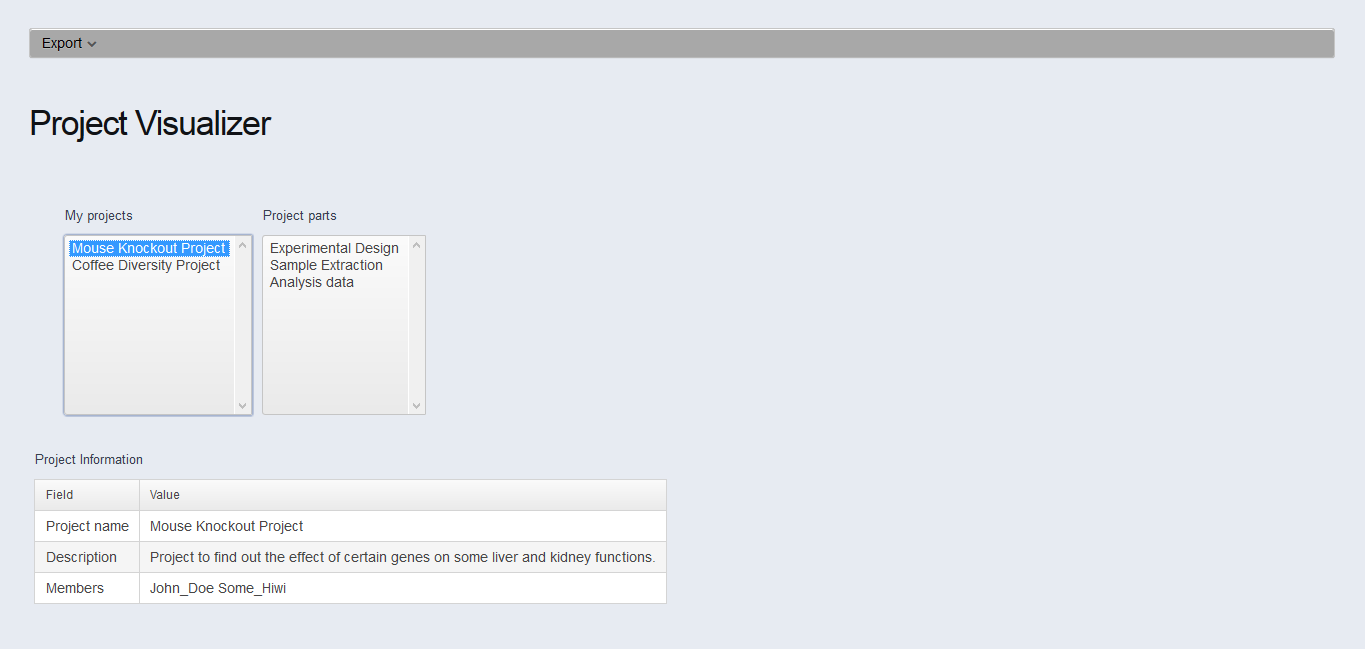
\includegraphics[scale=0.30]{GUI_1.png}
\caption[The GUI at the projet level]{The GUI at the project level. Here, users can make a decision between various available projects and inspect additional information.}
\label{fig:gui1}
\end{figure}
\noindent
If the user clicks on a specific experiment, two additional tables are visualized (Fig. \ref{fig:gui2_3}). One table showing available data files that are stored under a specific experiment and another one providing all existing experimental samples. The sample table has a multi selection feature, enabling the possibility to inspect the data sets that available for multiple samples. For instance, this can be seen in Fig. \ref{fig:gui2}. Here, two samples (QMOUS001A6 and QMOUS004AM) are selected, leading to a view at fastQ-files and quality control sites for each of the selected samples. All those datasets are click- and downloadable directly from the GUI.  
\begin{figure}[H]
\begin{subfigure}[b]{.45\linewidth}
\centering
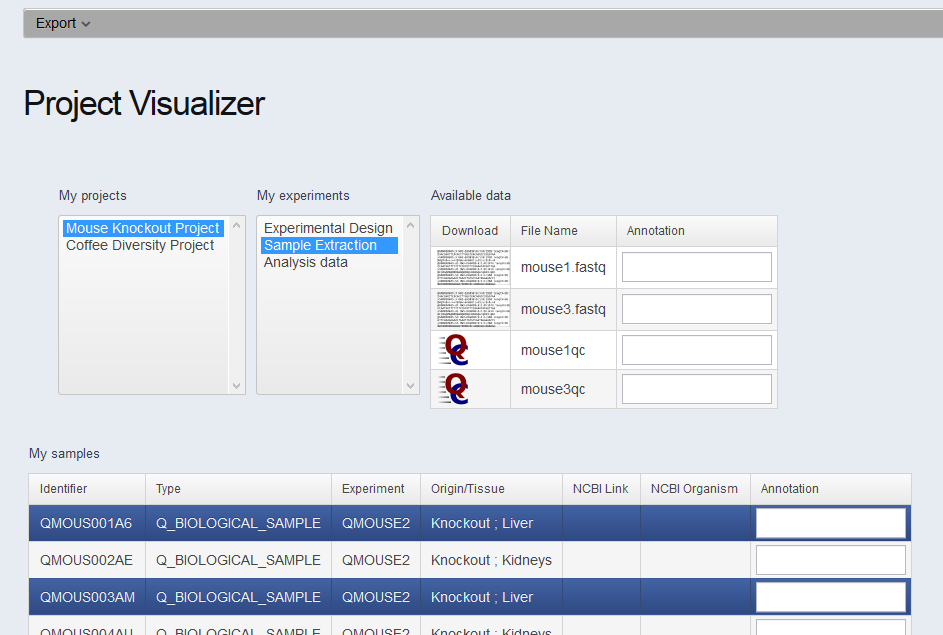
\includegraphics[scale=0.30]{GUI_2.png}
\caption{{Example for a experimental design.}}
\label{fig:gui2}
\end{subfigure}%
\quad
\begin{subfigure}[b]{.45\linewidth}
\centering
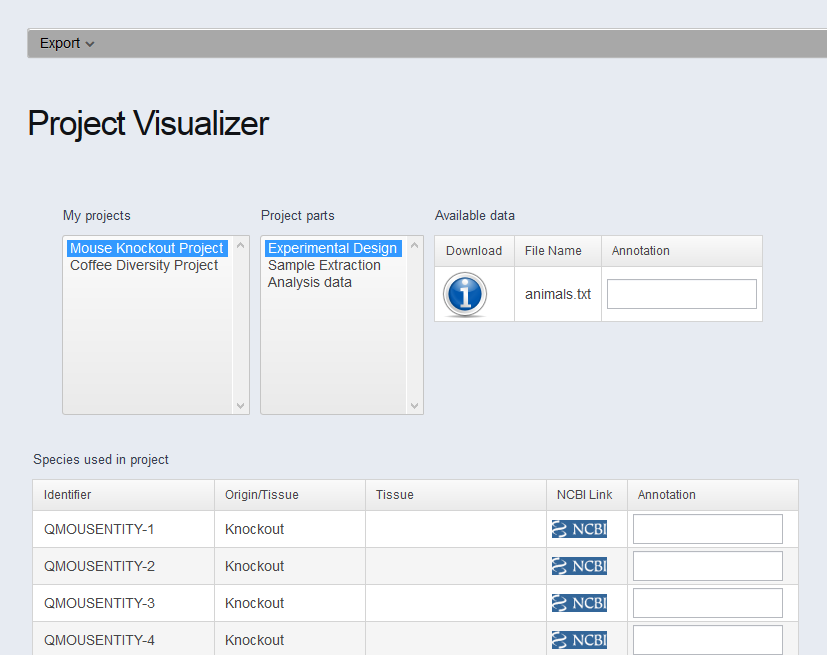
\includegraphics[scale=0.30]{GUI_3.png}
\caption{{Example for a sample extraction.}}
\label{fig:gui2}
\end{subfigure}%
\caption{The GUI at the sample level. Here, users can inspect the collection of samples together with stored data sets.}
\label{fig:gui2_3}
\end{figure}
\noindent
A additional feature is the possibility to add some annotations for samples and datasets behind each row. Here end-users might leave some additional information, that is later included into to report for exportation. Additionally, the sample table comes up with an external connection to the NCBI Taxonomy Browser \cite{Sayers01012009}, if an taxonomy ID is deposited for a sample (Fig. \ref{fig:gui2}). 
\subsection{Data Exporter}
With the aim to provide users with a printed summary of the visualized information, a data exporter has been developed. On clicking at the export menu bar, a new subwindow pops up, showing summarized information about a specific project in a new table. For instance, the project details, as well as the number of species together with their conditions for the specific experiments, are presented. As an extra feature, all samples/datasets, that have been annotated by the user, are also included together with their annotation into the summary table. An example for this can be seen in (Fig. \ref{fig:gui4}) based on the navigation and annotation of Fig. \ref{fig:gui2}). At the end, the user has two option in form of press-able buttons. One button exports the summary table in Excel format, the other one generates a PDF download.
\begin{figure}[H]
\centering
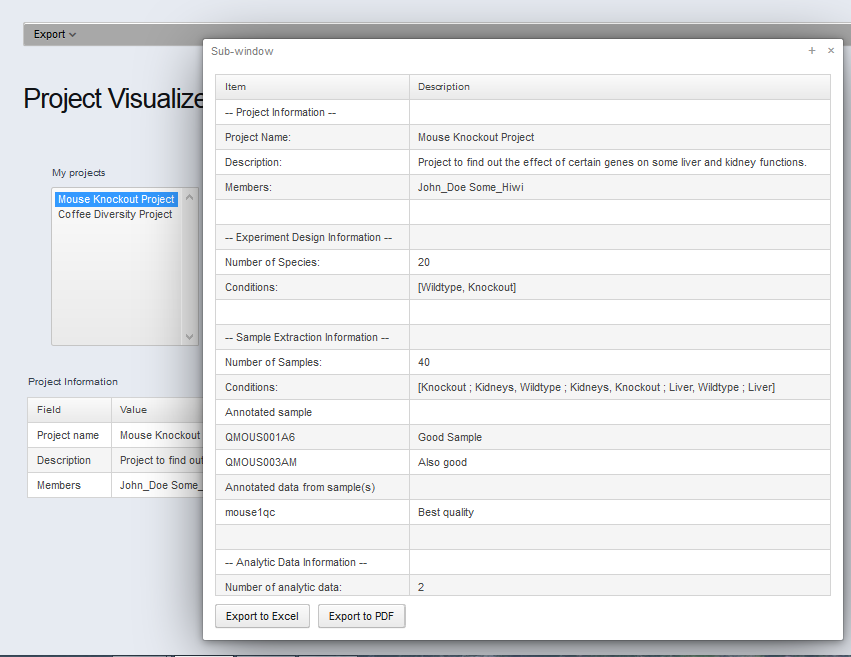
\includegraphics[scale=0.40]{GUI_4.png}
\caption[The export function]{The export function. Here, inspect and download a project summary in Excel or PDF format.}
\label{fig:gui4}
\end{figure}
\noindent 
\section{Discussion}
The complete project was structured in different phases. The first phase was the theoretical planning, how to visualize and integrate the data. Many questions arose in this phase, like: which data has to be visualised and which should not be visualised, how data is made easy accessible and what is a logic structure for a user to move through the file system.
In general only data serving for an effective information gain, is important to the user on a general interface. All other data, might be important for the program or further research, should not be visualized. Out of this statement results a new problem, as the decision between data for the program and biological information is easy, it is not easy to decide, what is more difficult to decide, what is additional information and what is information which should be visible on first sight. Respect to universality, we decided to visualize only information which is necessarily contained in each database. This is not an optimal information density on the gui, but the only possible. For further projects we would advice to define different experiment types. For example a mouse experiment, which shows the number of mice used or the wild types and so on.
Generally the databank design which was provided is discussable. One problem is, that there could be more than one Experiment for one project (like in figure1).   Our suggestion would be to add a new branch experiments between “My projects” and “Project pars”, which should get “experiment-parts”. To the new branch the experiment contents like design, samples and analysis should be outsourced to the experiment parts.
For the navigation through the database we decided to use a guide tree, which only shows the children of a node. This is in respect of the overview of the data. Different approaches like showing complete lists were neglected, because there would be to many rows.



Discussion of the columns, which are important for visualisation
What did we additional need ( IDs or stuff?)
How do we want to visualize, what is expected at the experiment level. how should users navigate.
Experiment subpoints
\bibliographystyle{unsrt}
\clearpage
\bibliography{ref}
\end{document}
